\documentclass[mathserif]{beamer}
%\documentclass[mathserif,handout]{beamer}
%\documentclass[dvips]{beamer}
\definecolor{Beige}{rgb}{0.96,0.96,0.86}
\definecolor{Yellow}{rgb}{1.,0.84,0.8}
\definecolor{Gold}{rgb}{1.,0.84,0.}
\definecolor{RedA}{hsb}{0.9,0.3,0.7}
\definecolor{RedB}{hsb}{0.9,0.3,1}
\definecolor{LightGray}{gray}{0.85}
\definecolor{Blue}{rgb}{0.,0.,1.}
\definecolor{Pink}{rgb}{0.9,0.75,0.8}
\definecolor{DarkGreen}{rgb}{1.0,1.0,1.0}
\definecolor{DarkBlue}{rgb}{0.,0.5,1.0}
%\definecolor{Pink}{rgb}{1.,0.75,0.8}
\definecolor{LightCyan}{rgb}{0.88,1.,1.}
%\definecolor{LightYellow}{rgb}{0.95,1.0,0.8}
\definecolor{red1}{rgb}{0.95,0.,0.}
%\definecolor{mycol1}{rgb}{0.9,0.2,0.9}
%\definecolor{mycol1}{rgb}{0.5,0.8,0.4}
\definecolor{mycol1}{rgb}{0.5,0.6,0.8}
\definecolor{mycol2}{rgb}{0.6,0.8,0.6}
\definecolor{LightYellow}{rgb}{0.95,1.0,0.8}

\mode<presentation>
{
%\usepackage{beamerthemeCambridgeUS, fancybox}
\usepackage{fancybox}
\usepackage{graphicx}
\usepackage{subfigure}
\usepackage[english]{babel}
\usepackage{multirow}
\usepackage{verbatim}
\usepackage{verbatim,epsfig,graphics,amssymb,amsmath,subfigure}
\usepackage{helvet}
\usepackage{graphicx}
\usepackage{wrapfig}
\setbeamercovered{transparent}
}
%\usepackage[T1]{fontenc}
%\usepackage[adobe-utopia]{mathdesign}
%\usepackage{fouriernc}
\usepackage[bitstream-charter]{mathdesign}
\usepackage[T1]{fontenc}



\usefonttheme{serif}

\usetheme{Boadilla} 

\setbeamertemplate{navigation symbols}{}
\setbeamersize{text margin left=3mm, text margin right=3mm}
\newcommand{\B}[1]{\boldsymbol{#1}}
\usepackage[all]{xy}
\usepackage[utf8]{inputenc}
%\usepackage{pdfpages}


\title[Seed-grant proposal]
{Multimodal classification of birds\\
\small{Seed-grant proposal}}

%\author[Paddy]{R. Padmanabhan (Paddy)}
\author[ADP]{Arnav Bhavsar\\
		Dileep A. D.\\
		Padmanabhan Rajan
}

\institute[IIT Mandi] {
Multimedia Analytics and Systems Lab\\
School of Computing and Electrical Engineering\\
%Indian Institute of Technology Mandi \\

\includegraphics[width=4cm,height=2cm]{figures/mas_logo.pdf}

\includegraphics[width=3cm,height=2cm]{figures/iitmandi-logo.pdf}
}
%\date[November 11th, 2009]
{}

%%%%%%%%%%%%%%%%%%%%%%%%%%%%%%%%%%%%%%%%%%%%%%%%%%%%%%%%%%%%%%%%%%%%%%%%%%%%%%%%%%%%%%%%%%%%%
\begin{document}
\normalfont

%%%%%%%%%%%%%%%%%%%%%%%%%%%%%%%%%%%%%%%%%%%%%%%%%%%%%%%%%%%%%%%%%%%%%%%%%%%%%%%%
\begin{frame}
        \titlepage
\end{frame}

%\logo{
\includegraphics[height=0.8cm]{figures/iitmandi-logo.pdf}\vspace{220pt}}
\logo{
\includegraphics[height=0.8cm]{figures/mas_logo.pdf}\vspace{220pt}}

\begin{frame}
\frametitle{Overview}
\begin{wrapfigure}{r}{0.5\textwidth}
\centering
%  \begin{center}
    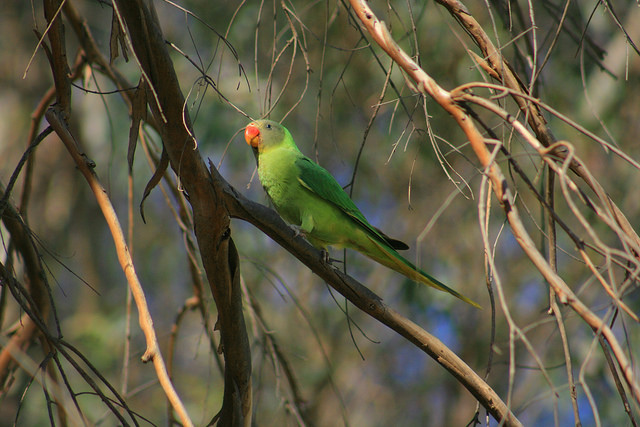
\includegraphics[width=0.48\textwidth]{figures/parakeet.jpg}
%  \end{center}
  \caption{\small{Slaty-headed parakeet. Pic by PPJ.}}
\end{wrapfigure}
The objective\\
The acoustics\\
The image/video\\
The machine learning\\
The budget and other details\\
\end{frame}

\begin{frame}
\frametitle{The objective}
\begin{itemize}
\item<2-> Develop algorithms for automatic analysis of avain biodiversity
\item<3-> Combine information from acoustic and visual data streams
\item<4-> Sensors: microphones, cameras
\item<5-> Apply signal processing and machine-learning techniques to collected
data
\item<6-> Tasks: Species identification, species detection
\end{itemize}
\end{frame}

\begin{frame}
\frametitle{The motivation}
\begin{itemize}
\item<2-> Birds provide crucial ecosystem services: pollination, seed dispersal,
insectivory
\item<3-> Avian diversity: good indicator of ecosystem health in a local area
\item<4-> Automatic and semi-automatic sensing devices can be utilised
\item<5-> Large volume of data captured by these devices
\item<6-> Algorithms to analyse this data would be useful to ecologists
\item<7-> Our campus location in the lower Himalays: sensitive ecosystem
\item<8-> Proposed system can be used for long-term ecological monitoring
\end{itemize}
\end{frame}

\begin{frame}
\frametitle{The challenges}
\begin{itemize}
\item<2-> Challenges at various levels
\item<3-> Acoustics:
	\begin{itemize}
	\item<4-> Complex acoustic environment where recordings are made
	\item<5-> Overlapping vocalisations, intra-species call variability
	\item<7-> Background sounds (other animals, human-made sounds, river etc.)
	\end{itemize}
\item<8-> Image/video 
	\begin{itemize}
	\item<9-> Complex visual environment, visual background clutter
	\item<10-> Overlapping inter-class visual appearances, local variations  
	\item<11-> Intra-class variations: Robustness to changes in pose, motion, light conditions.
	\end{itemize}
\item<12-> Fusion of modalities
	\begin{itemize}
	\item<13-> Curating of feature vectors and subsystem decisions 
	\item<14-> Complementary representations from different modalities
	\item<15-> Correlating sound and videos
	\end{itemize}
\item<15-> Machine-learning
	\begin{itemize}
	\item<16-> Fixed-length representations
	\item<17-> Bag-of-features
	\end{itemize}
\end{itemize}
\end{frame}


\begin{frame}
\frametitle{The acoustics}
\vspace{-1cm}
Automatic analysis of birdcalls: fairly active research area\\
\vspace{0.3cm}
\pause
Data acquisition: rugged, field-deployable recorders \\
eg.~Song Meter SM3 recorder from Wildlife Acoustics Inc, USA.
\begin{wrapfigure}{r}{0.3\textwidth}
	\centering
	\only<2>{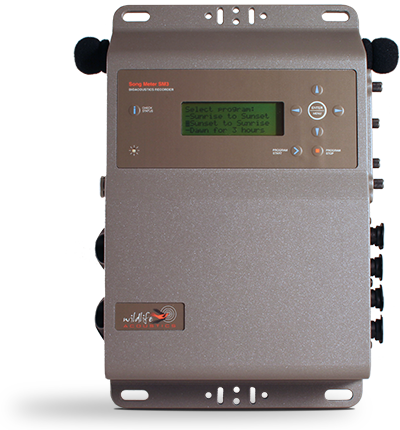
\includegraphics[width=0.3\textwidth]{figures/songMeter.png}}
	%\caption{\small{Song Meter SM3 recorder}}
\end{wrapfigure}
\end{frame}


\begin{frame}
\frametitle{The acoustics (cont'd)}
\begin{itemize}
\item<2-> Processing of human speech: techniques can be adapted for birdcalls
\item<3-> Production mechanims are different, but have similarities (eg. formant
structure)
\item<4-> Existing techniques include:
\begin{itemize}
	\item spectral representations \footnote{
	H. Tyagi et. al., ``Automatic identification of bird calls using spectral 
	ensemble average voice prints'', Proc. EUSIPCO, 2006},
	\item Mel frequency cepstra \footnote{M. Graciarena et. al., 
	``Acoustic front-end optimization for bird species recognition'', 
	Proc. ICASSP, 2010}, 
	\item hidden Markov models \footnote{M. Graciarena et.al., 
	``Bird species recognition combining acoustic and sequence modeling'', 
	Proc. ICASSP, 2011}, 
	\item sparse representations \footnote{L. N. Tan et. al. 
	``Evaluation of a sparse representation-based classifier for bird phrase 
	classification", Proc. Interspeech, 2012}
\end{itemize}
\end{itemize}
\end{frame}


\begin{frame}
\frametitle{The acoustics (cont'd)}
\begin{itemize}
\item<2-> Research focus: \textcolor{blue}{subspace representations} 
\item<3-> A recording can be represented as a fixed-length vector $\mathbf{x}$ 
\item<4-> Can be used for various applications, for eg. removing background
sounds before classification:
\begin{itemize}
	\item<5-> Project $\mathbf{x}$ into a subspace of background sounds, and remove this
	component from $\mathbf{x}$
\end{itemize}
\item <6-> Fixed-length representations: utilised in kernel functions for
support vector machines
\end{itemize}
\end{frame}


\begin{frame}
\frametitle{The visual: Research areas}
\begin{itemize}
\item<2-> Fine-grained classification (of birds): Relatively recent research area ($\geq$ 2010)
\item<3-> Detection, segmentation and tracking of birds (relatively unexplored): \\Adapting general object detection, segmentation and tracking methods.
\item<4-> Learning visual guidance: Inverse problem to classification \\$\Rightarrow$ Given the classes, find the discriminative features
\item<5-> Sound source localization (active area in general domains): \\Challenges for birds: less visual motion, background sounds
\end{itemize}
\end{frame}


\begin{frame}
\footnotesize
\frametitle{The visual: Existing work}
\begin{itemize}
	\item<2-> Fine-grained classification 
	\begin{itemize}
	\footnotesize
	\item H. Tyagi et. al., ``Automatic identification of bird calls using spectral 
	ensemble average voice prints'', Proc. EUSIPCO, 2006,
	\item M. Graciarena et. al., ``Acoustic front-end optimization for bird species recognition'', 
	Proc. ICASSP, 2010, 
	\item M. Graciarena et.al., ``Bird species recognition combining acoustic and sequence modeling'', 
	Proc. ICASSP, 2011, 
	\end{itemize}	
	\item<3-> Visual guidance: 
	\item<4-> Detection, Segmentation
	\begin{itemize}
	\footnotesize
	\item H. Tyagi et. al., ``Automatic identification of bird calls using spectral 
	ensemble average voice prints'', Proc. EUSIPCO, 2006,
	\item M. Graciarena et. al., ``Acoustic front-end optimization for bird species recognition'', 
	Proc. ICASSP, 2010, 
	\item M. Graciarena et.al., ``Bird species recognition combining acoustic and sequence modeling'', 
	Proc. ICASSP, 2011, 
	\end{itemize}
\end{itemize}
\end{frame}

\begin{frame}
\frametitle{The visual: Possible directions}
\begin{itemize}
\item<2-> Features and frameworks: 
\begin{itemize}
\item Patch-based features 
\item Body-part features: Appearance and Geometric relationships
\item Feature learning: Deep neural networks, Discriminative features
\end{itemize}
\item<3-> Frameworks:
\begin{itemize}
\item Sparse representation
\item Markov Random Fields
\item Hierarchical classification 
\end{itemize}
\item<4-> Systems:
\begin{itemize}
\item Dataset collection
\item Audio-video systems for monitoring
\item On-board algorithms: Detection, tracking
\end{itemize}
\end{itemize}
\end{frame}


\begin{frame}
\frametitle{The machine learning}
\begin{itemize}
\item<2-> Machine learning teching for bird image identification
\item<3-> Bird classification: techniques can be adapted for birdcalls
\item<4-> Production mechanisms are different, but have similarities (eg. formant
structure)
\item<5-> Existing techniques include:
\begin{itemize}
	\item spectral representations \footnote{
	H. Tyagi et. al., ``Automatic identification of bird calls using spectral 
	ensemble average voice prints'', Proc. EUSIPCO, 2006},
	\item Mel frequency cepstra \footnote{M. Graciarena et. al., 
	``Acoustic front-end optimization for bird species recognition'', 
	Proc. ICASSP, 2010}, 
	\item hidden Markov models \footnote{M. Graciarena et.al., 
	``Bird species recognition combining acoustic and sequence modeling'', 
	Proc. ICASSP, 2011}, 
	\item sparse representations \footnote{L. N. Tan et. al. 
	``Evaluation of a sparse representation-based classifier for bird phrase 
	classification", Proc. Interspeech, 2012}
\end{itemize}
\end{itemize}
\end{frame}


\begin{frame}
\frametitle{Budget and other details}

\begin{table}[th]
\centering
\caption{Projected expenses in lakhs INR.}
\begin{tabular}{|c|c|c|c|c|}
\hline
Items & Year 1 & Year 2 & Year 3 & Total\\
\hline
High-end computers (2) & 3.0 & 3.0 & 0 & 6.0\\
Imaging and audio equipment & 5.0 & 3.0 & 0 & 8.0 \\
Desktop computers (6) & 5.0 & 0 & 0 & 5.0  \\
Contingency & 0.5 & 0.5 & 1.0 & 2.0 \\
Travel & 0.5 & 0.5 & 1.0 & 2.0\\
\hline
Overall & 15.0 & 8.0 & 2.0 & \textbf{23.0} \\
\hline
\end{tabular}
\label{tab:funding}
\end{table}
\end{frame}


\begin{frame}
\frametitle{Future plans: Further funding}
\begin{itemize}
\item \textbf{Proposal to SERB (ready for submission)}:
\item \textbf{Proposal planned:} Camera and acoustic sensor networks for a local area (IIT Mandi campus)
\end{itemize}
\end{frame}


\begin{frame}
\frametitle{}
\Large{Thank you for your attention.}
\end{frame}


\end{document}

